\documentclass[a4paper]{article}

\usepackage{geometry}
\geometry{margin=2.5cm}

\usepackage[utf8]{inputenc}
\usepackage{polski}
\usepackage[polish]{babel}

\usepackage{graphicx} % Required for inserting images
\usepackage{placeins} % For \FloatBarrier
\usepackage{siunitx}
\usepackage{amsmath}
\numberwithin{equation}{section} % Numeracja rownan

\renewcommand{\arraystretch}{1.5}

\title{Mechanika Ogólna --- materiały do zajęć}
\author{Paweł Bielski, WIMiO PG}
\date{\today}

\begin{document}

\maketitle
\tableofcontents

\section{Podstawy rachunku wektorowego}

\subsubsection*{Skalar}

\begin{equation}
    a
\end{equation}

\subsubsection*{Wektor}

\begin{equation}
    \Vec{a} = [ a_x;\ a_y;\ a_z ] = \begin{bmatrix} a_x \\ a_y \\ a_z \end{bmatrix}
\end{equation}

\subsubsection*{Punkt}

\begin{equation}
    O( O_x;\\ O_y;\\ O_z )
\end{equation}

\subsubsection*{Suma wektorów}

\begin{equation}
    \Vec{a} + \Vec{b} = [ a_x + b_x;\ a_y + b_y;\ a_z + b_z ]
\end{equation}

\subsubsection*{Iloczyn skalarny}

\begin{equation}
    \Vec{a} \cdot \Vec{b} = a_x b_x + a_y b_y + a_z b_z
\end{equation}

\begin{equation}
    \Vec{a} \cdot \Vec{b} = |\Vec{a}| |\Vec{b}| \cos\alpha
\end{equation}

\subsubsection*{Moduł wektora}

\begin{equation}
    |\Vec{a}| = \sqrt{\Vec{a} \cdot \Vec{a}} = \sqrt{ a_x^2 + a_y^2 + a_z^2 }
\end{equation}

\subsubsection*{Wersor}

\begin{equation}
    \Vec{e} = [ e_x;\ e_y;\ e_z ]
\end{equation}

\begin{equation}
    |\Vec{e}| = \sqrt{\Vec{e} \cdot \Vec{e}} = \sqrt{ e_x^2 + e_y^2 + e_z^2 } = 1
\end{equation}

\subsubsection*{Wersor bazowy}

\begin{align}
    \Vec{i} = [1;\ 0;\ 0] \nonumber \\
    \Vec{j} = [0;\ 1;\ 0] \nonumber \\
    \Vec{k} = [0;\ 0;\ 1]
\end{align}

\subsubsection*{Inne zapisy wektora}

\begin{equation}
    \Vec{a} = a_x \Vec{i} + a_y \Vec{j} + a_z \Vec{k}
\end{equation}

\begin{equation}
    \Vec{a} = a \Vec{e}_a = a [ e_{a,x};\ e_{a,y};\ e_{a,z} ]
\end{equation} % Rachunek wektorowy
\input{Text/P1} \FloatBarrier % Przyklady z rachunku wektorowego
\newpage

\section{Siły i momenty w przestrzeni wektorowej}

\subsubsection*{Iloczyn wektorowy}

\begin{equation}
    \Vec{c} = \Vec{a} \times \Vec{b} = \begin{vmatrix}
    \Vec{i} & \Vec{j} & \Vec{k} \\
    a_x & a_y & a_z \\
    b_x & b_y & b_z
    \end{vmatrix}  = \Vec{i}(a_y b_z - a_z b_y) - \Vec{j}(a_x b_z - a_z b_x) + \Vec{k}(a_x b_y - a_y b_x)
\end{equation}

\begin{equation}
    \Vec{c} = [a_y b_z - a_z b_y;\ a_z b_x - a_x b_z;\ a_x b_y - a_y b_x]
\end{equation}

\begin{equation}
    |\Vec{c}| = |\Vec{a}| |\Vec{b}| \sin\alpha
\end{equation}

\subsubsection*{Moment siły względem punktu}

Punkt, względem którego liczymy moment siły:

\begin{equation*}
    O(O_y;\ O_z;\ O_z)
\end{equation*}

Punkt zaczepienia siły:

\begin{equation*}
    A(A_y;\ A_z;\ A_z)
\end{equation*}

Ramię siły:

\begin{equation}
    \Vec{r} = \Vec{OA} = [A_x - O_x;\ A_y - O_y;\ A_z - O_z]
\end{equation}

Siła:

\begin{equation*}
    \Vec{F} = [F_x;\ F_y;\ F_z]
\end{equation*}

Moment siły względem punktu:

\begin{equation}
    \Vec{M}_{O,F} = \Vec{r} \times \Vec{F} = \begin{vmatrix}
    \Vec{i} & \Vec{j} & \Vec{k} \\
    r_x & r_y & r_z \\
    F_x & F_y & F_z
    \end{vmatrix}
\end{equation}

\subsubsection*{Redukcja układu do punktu}

Siła główna:

\begin{equation}
    \Vec{F}_0 = \sum \Vec{F}_i = \left[ \sum F_{i,x};\ \sum F_{i,y};\ \sum F_{i,z} \right]
\end{equation}

Moment główny:

\begin{equation}
    \Vec{M}_0 = \sum \Vec{r}_i \times \Vec{F}_i + \sum \Vec{M}_j
\end{equation}

gdzie $i$ - liczba sił skupionych w układzie, $j$ - liczba momentów skupionych w układzie.

\subsubsection*{Warunek równowagi statycznej}

\begin{equation}
    \begin{cases}
        \Vec{F}_0 = \Vec{0} \\
        \Vec{M}_0 = \Vec{0}
    \end{cases}
\end{equation}

\begin{equation}
    \begin{cases}
        F_{0,x} = 0 \\
        F_{0,y} = 0 \\
        F_{0,z} = 0 \\
        M_{0,x} = 0 \\
        M_{0,y} = 0 \\
        M_{0,z} = 0
    \end{cases}
\end{equation} % Rownowaga sil
\subsection*{Zadania: redukcja układu sił i momentów}

\subsubsection*{Zadanie 1}

Narysuj układ sił $F_i$ zaczepionych w punktach $A_i$. Wyznacz moment główny od tych sił w punkcie $C(3,3,0)\si{m}$.

\begin{equation*}
    \begin{cases}
        A_1(3;\ 5;\ 0) \\
        A_2(4.414;\ 4.414;\ 0) \\
        A_3(5;\ 3;\ 0) [ \si{m} ]
    \end{cases}
    \qquad
    \begin{cases}
        \Vec{F}_1 = [2;\ 0;\ 0 ] \\
        \Vec{F}_2 = [1.414;\ -1.414;\ 0 ] \\
        \Vec{F}_3 = [0;\ -2;\ 0 ] [ \si{kN} ]
    \end{cases}
\end{equation*}

\subsubsection*{Zadanie 2}

Narysuj układ sił $F_i$ zaczepionych w punktach $A_i$. Wyznacz moment główny od tych sił w punkcie $C(4,2,0)\si{m}$.

\begin{equation*}
    \begin{cases}
        A_1(0;\ 4;\ 0) \\
        A_2(4;\ 4;\ 0) \\
        A_3(8;\ 4;\ 0) [ \si{m} ]
    \end{cases}
    \qquad
    \Vec{F}_1 = \Vec{F}_2 = \Vec{F}_3 = [2;\ 0;\ 0] \si{kN}
\end{equation*}

\subsubsection*{Zadanie 3}

Narysuj układ sił $F_i$ i momentów $M_j$ zaczepionych w punktach $A_i,A_j$. Zredukuj układ do punktu $O(0,0,0)$.

\begin{equation*}
    \begin{cases}
        A_1(3;\ 2;\ 0) \\
        A_2(0;\ 3;\ 4) \\
        A_3(2;\ 0;\ 4) \\
        A_4( 0;\ 2;\ 4 ) \\
        A_5(0;\ 5;\ 0) [ \si{m} ]
    \end{cases}
    \qquad
    \begin{cases}
        \Vec{F}_1 = [ 5;\ 5;\ 0 ] \\
        \Vec{F}_2 = [ 10;\ 0;\ 0 ] \\
        \Vec{F}_3 = [ 0;\ -10;\ 0 ] \\
        \Vec{F}_4 = [-5;\ 0;\ 5] [ \si{kN} ] \\
        \Vec{M}_5 = [0;\ 0;\ 40] \si{kNm}
    \end{cases}
\end{equation*} \FloatBarrier % Zadania z redukcji sil
\newpage

\section{Środki ciężkości}

\subsubsection*{Średnia ważona}

\begin{equation}
    x_{sr} = \dfrac{\sum w_i x_i}{\sum w_i}
\end{equation}
gdzie $w_i$ oznacza wagi, $x_i$ ważone wielkości, a $x_{sr}$ średnią ważoną

\subsubsection*{Środek ciężkości układu mas skupionych}

\begin{equation}
    x_c = \dfrac{\sum m_i x_i}{\sum m_i}
\end{equation}

\[
    y_c = \dfrac{\sum m_i y_i}{\sum m_i}
\]

\[
    z_c = \dfrac{\sum m_i z_i}{\sum m_i}
\]

\subsubsection*{Środek ciężkości figur i brył jednorodnych}

W przypadku figur płaskich:

\begin{equation}
    x_c = \dfrac{\sum A_i x_i}{\sum A_i}
\end{equation}

\[
    y_c = \dfrac{\sum A_i y_i}{\sum A_i}
\]
gdzie $A_i$ oznacza pole powierzchni danej figury składowej.

W przypadku brył:

\begin{equation}
    x_c = \dfrac{\sum V_i x_i}{\sum V_i}
\end{equation}

\[
    y_c = \dfrac{\sum V_i y_i}{\sum V_i}
\]

\[
    z_c = \dfrac{\sum V_i z_i}{\sum V_i}
\]
gdzie $V_i$ oznacza objętość danej bryły składowej.

\subsubsection*{Środek ciężkości figur i brył niejednorodnych}

W przypadku figur płaskich:

\begin{equation}
    x_c = \dfrac{\sum \gamma_i A_i x_i}{\sum \gamma_i A_i}
\end{equation}

\[
    y_c = \dfrac{\sum \gamma_i A_i y_i}{\sum \gamma_i A_i}
\]
gdzie $\gamma_i$ oznacza ciężar powierzchniowy [kN/m$^2$] danej figury składowej.

W przypadku brył:

\begin{equation}
    x_c = \dfrac{\sum \gamma_i V_i x_i}{\sum \gamma_i V_i}
\end{equation}

\[
    y_c = \dfrac{\sum \gamma_i V_i y_i}{\sum \gamma_i V_i}
\]

\[
    z_c = \dfrac{\sum \gamma_i V_i z_i}{\sum \gamma_i V_i}
\]
gdzie $\gamma_i$ oznacza ciężar objętościowy [kN/m$^3$] danej bryły składowej. % Srodki ciezkosci
\subsection*{Zadania: Środki ciężkości}

Wyznacz położenie środków ciężkości płaskich arkuszy blach. W przypadku blach niejednorodnych uwzględnij różnicę w rozkładzie ciężaru powierzchniowego $\gamma$.

\begin{figure}[htbp]
    \centering
    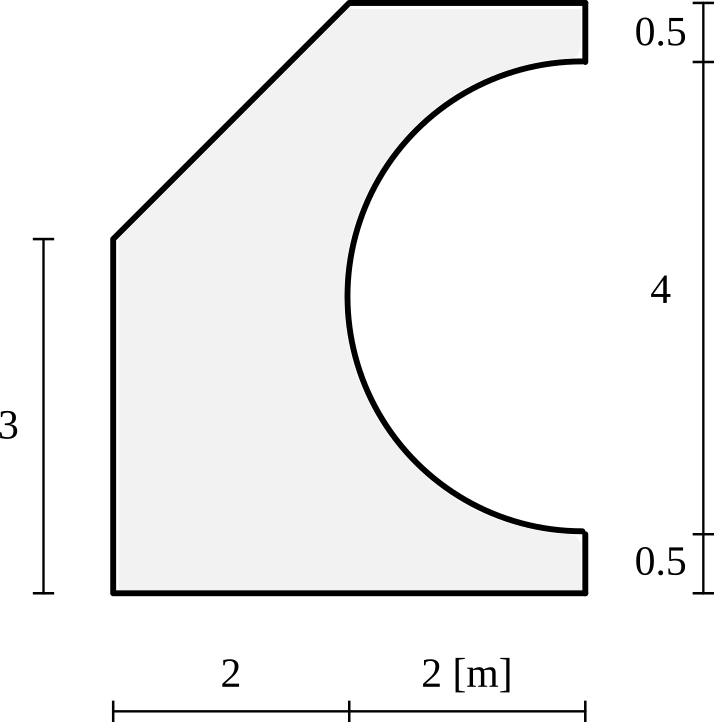
\includegraphics{SrodkiCiezkosci/Figura01.png}
    \caption{Blacha jednorodna z wycięciem}
\end{figure}

\begin{figure}[htbp]
    \centering
    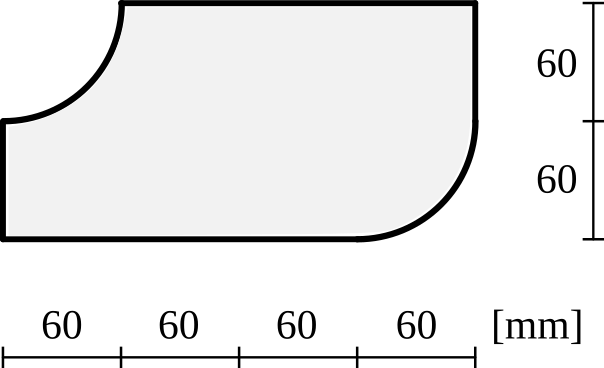
\includegraphics{SrodkiCiezkosci/Figura02.png}
    \caption{Blacha jednorodna z zaokrągleniami}
\end{figure}

\begin{figure}[htbp]
    \centering
    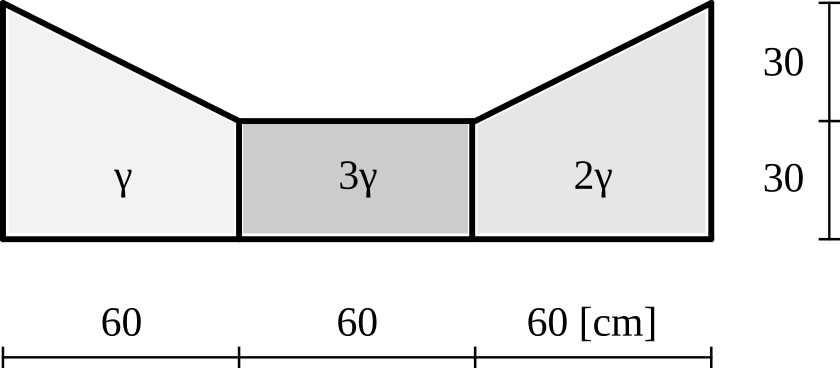
\includegraphics{SrodkiCiezkosci/Figura03.png}
    \caption{Blacha niejednorodna}
\end{figure}

\begin{figure}[htbp]
    \centering
    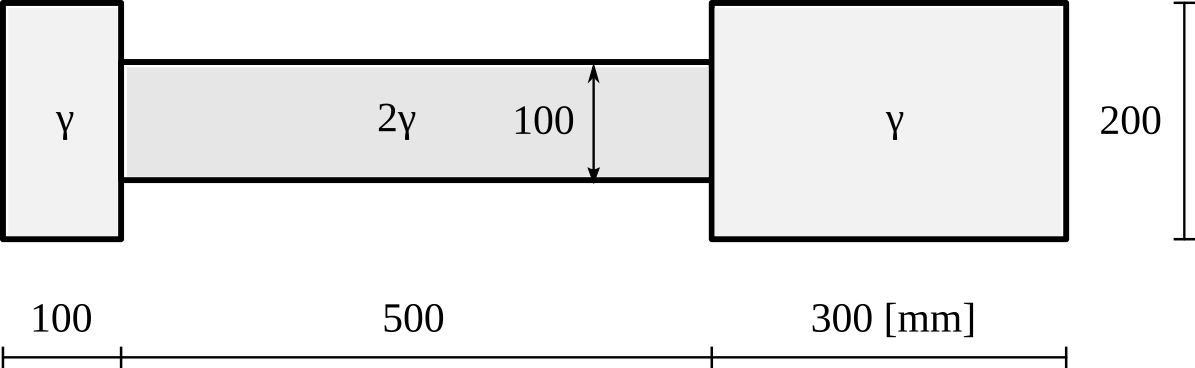
\includegraphics{SrodkiCiezkosci/Figura04.png}
    \caption{Blacha niejednorodna}
\end{figure} \FloatBarrier % Zadania ze srodkow ciezkosci
\newpage

\section{Reakcje podporowe w układach płaskich}

\subsection*{Warunek równowagi}

Reakcje wyznaczamy z warunku równowagi statycznej:

\begin{equation}
    \begin{cases}
        \Vec{F}_0 = \Vec{0} \\
        \Vec{M}_0 = \Vec{0}
    \end{cases}
\end{equation}
który w płaskim układzie sił przyjmuje postać:

\begin{equation}
    \begin{cases}
        F_{0,x} = 0 \\
        F_{0,y} = 0 \\
        M_{0,z} = 0
    \end{cases}
\end{equation}

\subsection*{Układ dwóch sił i momentu skupionego}

Jeżeli reakcje stanowi układ dwóch wektorów sił i jegnego momentu skupionego:
\begin{itemize}
    \item Równanie momentów rozpisujemy względem punktu $A$, w którym przecinają się osie działania wektorów sił - z tego równania wyznaczamy wartość momentu skupionego,
    \item Wartości sił uzyskujemy z równań zerowania się rzutów sił na kierunkach $x$ i $y$.
\end{itemize}

\begin{equation}
    \begin{cases}
        \sum M_z^A = 0 \\
        \sum F_x = 0 \\
        \sum F_y = 0
    \end{cases}
\end{equation}

Jeżeli reakcje stanowi układ trzech wektorów sił:
\begin{itemize}
    \item Równanie momentów rozpisujemy względem punktów $A$ i $B$, w których przecinają się osie działania wektorów sił - z tych równania wyznaczamy dwie z trzech niewiadomych sił,
    \item Trzecią siłę uzyskujemy z równania zerowania się rzutów sił na kierunku $x$ lub $y$,
    \item Ostatnie równanie (suma rzutów sił na kierunku $x$ lub $y$) traktujemy jako równanie sprawdzające.
\end{itemize}

\begin{equation}
    \begin{cases}
        \sum M_z^A = 0 \\
        \sum M_z^B = 0 \\
        \sum F_x = 0 \\
        \sum F_y = 0
    \end{cases}
\end{equation} % Reakcje podporowe
\subsection*{Zadania: Reakcje podporowe}

Wyznacz reakcje podporowe w poniższych przykładach. Uwzględnij ciężar własny tarczy tam, gdzie podany jest ciężar powierzchniowy. W pozostałych przypadkach pomiń go.

\begin{figure}[htbp]
    \centering
    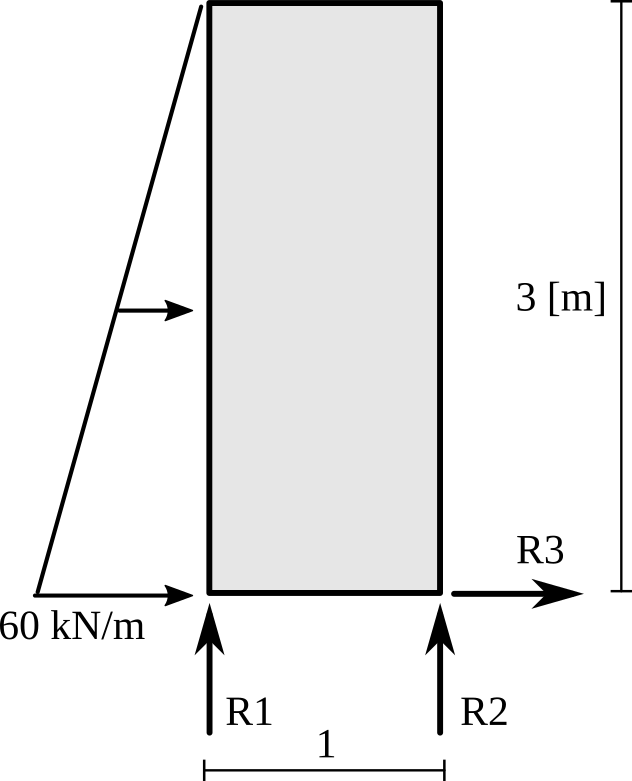
\includegraphics{Reakcje/Tarcza01.png}
    \caption{Układ A - obciążenie rozłożone trójkątne}
\end{figure}

\begin{figure}[htbp]
    \centering
    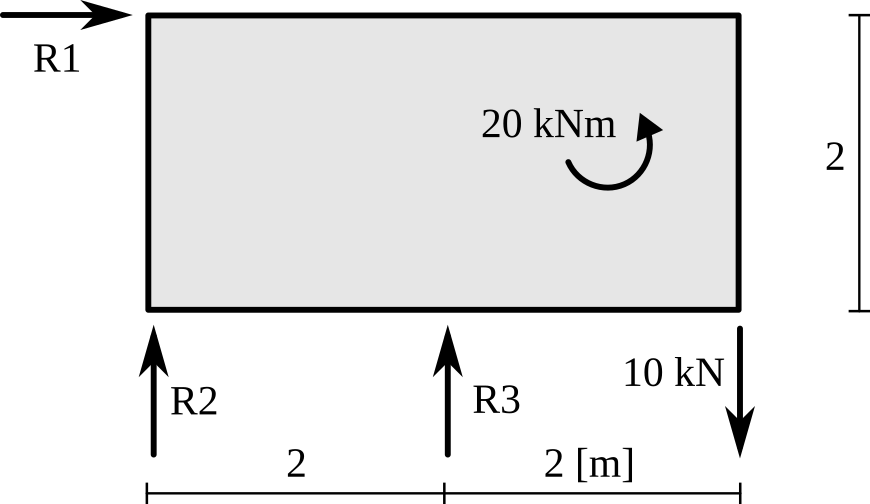
\includegraphics{Reakcje/Tarcza02.png}
    \caption{Układ B - siły i momenty skupione}
\end{figure}

\begin{figure}[htbp]
    \centering
    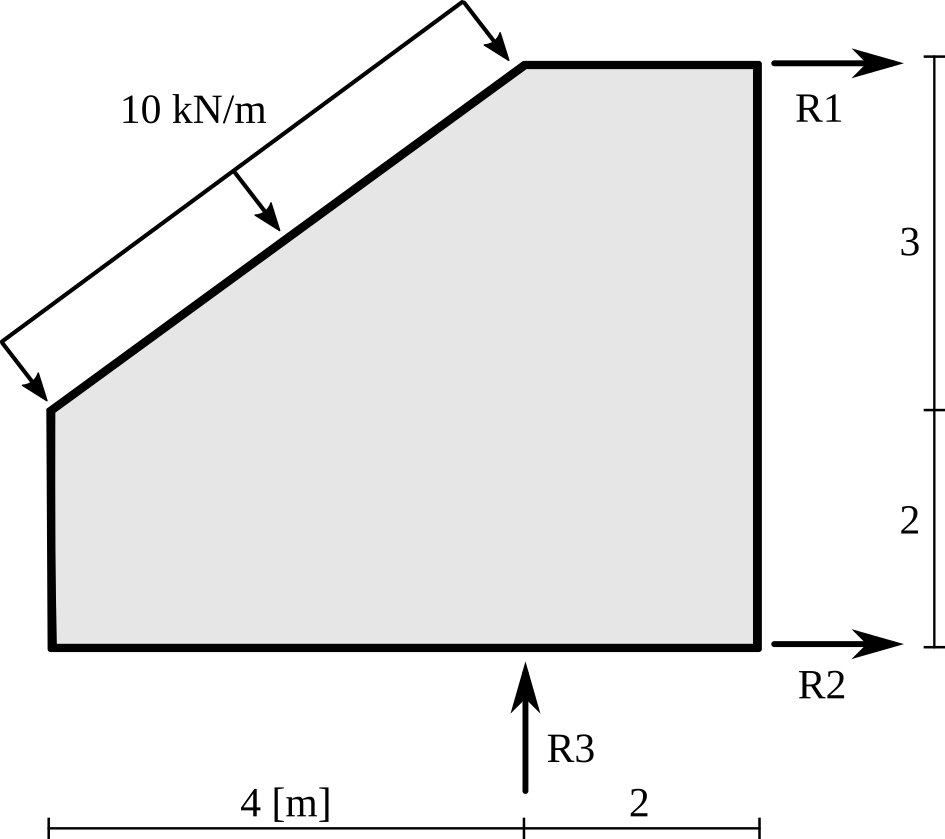
\includegraphics{Reakcje/Tarcza03.png}
    \caption{Układ C - obciążenie rozłożone na odcinku ukośnym}
\end{figure}

\begin{figure}[htbp]
    \centering
    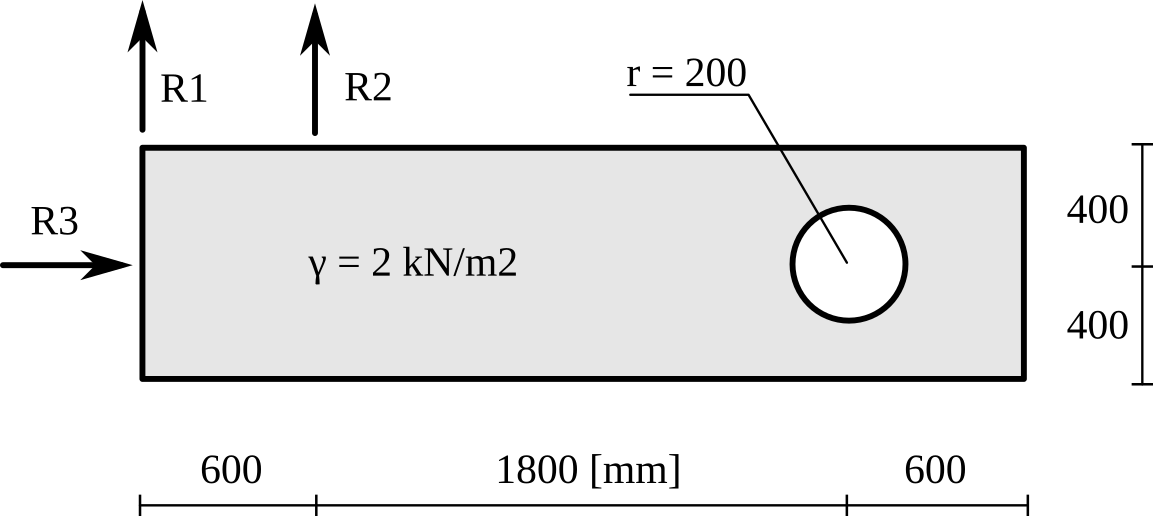
\includegraphics{Reakcje/Tarcza04.png}
    \caption{Układ D - ciężar własny}
\end{figure} \FloatBarrier % Zadania z reakcji podporowych
\subsection*{Zadania: Siły wewnętrzne w kratownicach}

W poniższych układach wyznacz wykresy sił normalnych

\begin{figure}[htbp]
    \centering
    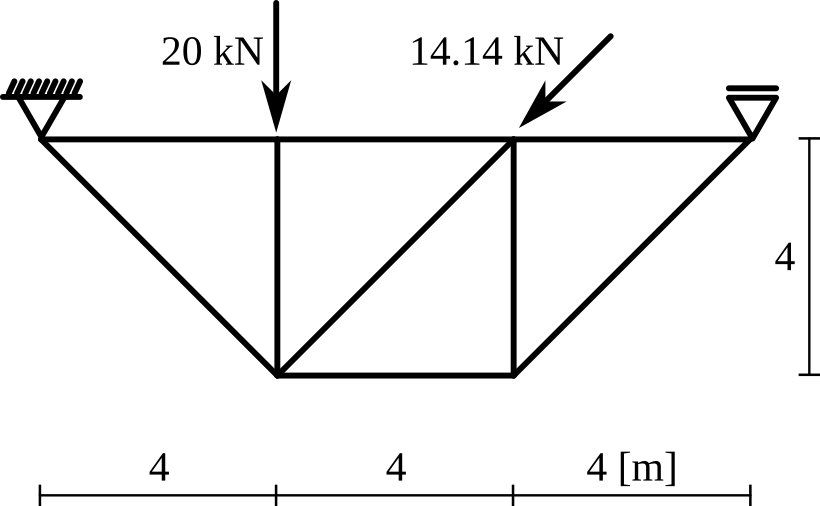
\includegraphics{Kratownice/Truss01.png}
    %\caption{}
\end{figure}

\begin{figure}[htbp]
    \centering
    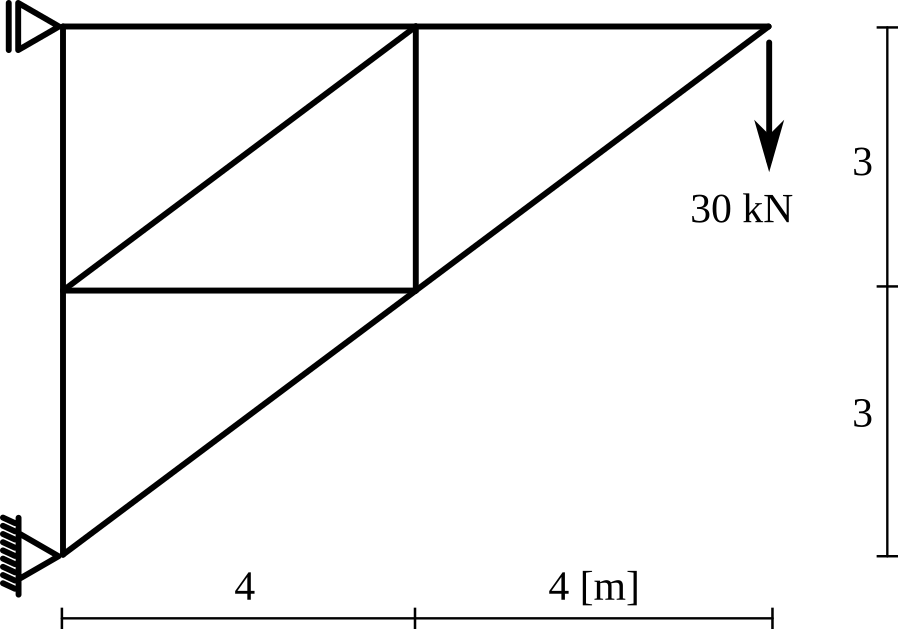
\includegraphics{Kratownice/Truss02.png}
    %\caption{}
\end{figure}

\begin{figure}[htbp]
    \centering
    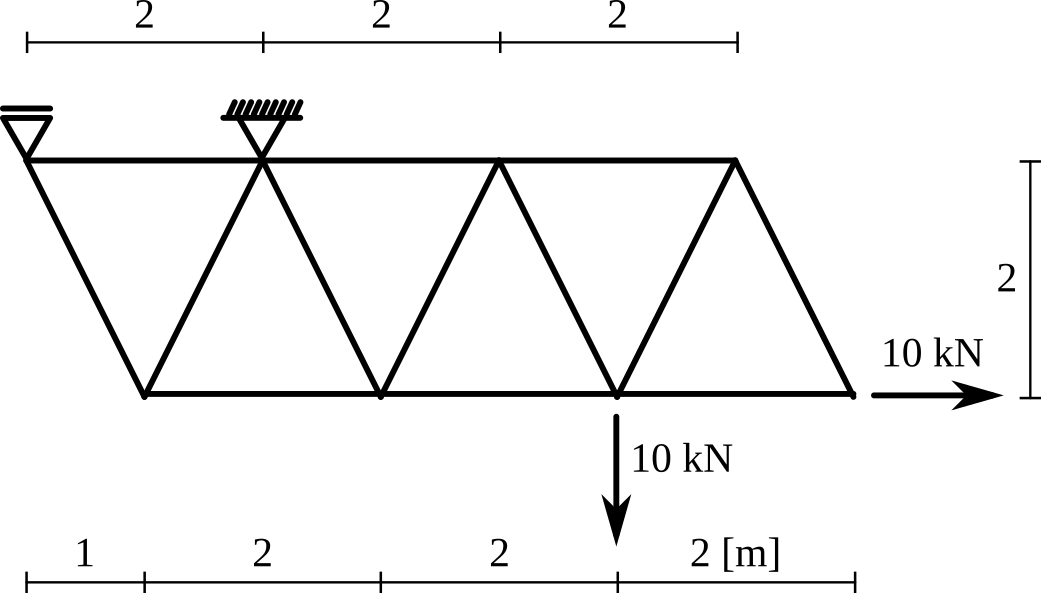
\includegraphics{Kratownice/Truss03.png}
    %\caption{}
\end{figure}

\begin{figure}[htbp]
    \centering
    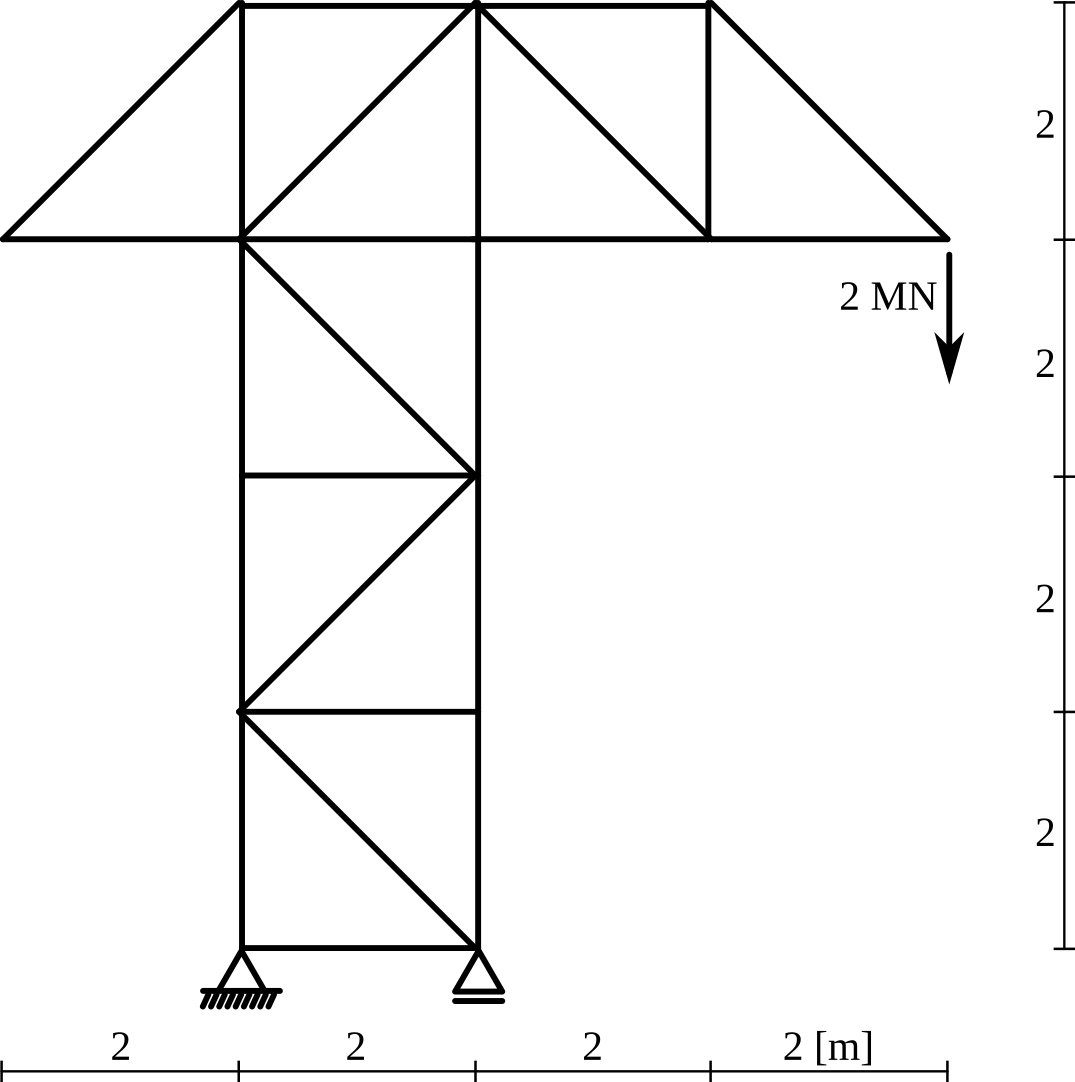
\includegraphics{Kratownice/Truss04.png}
    %\caption{}
\end{figure} \FloatBarrier % Zadania z sil w kratownicach
\newpage

%\subsection*{Zadania: Siły wewnętrzne w belkach}

W poniższych układach wyznacz wykresy sił normalych, tnących oraz momentów zginających

\begin{figure}[htbp]
    \centering
    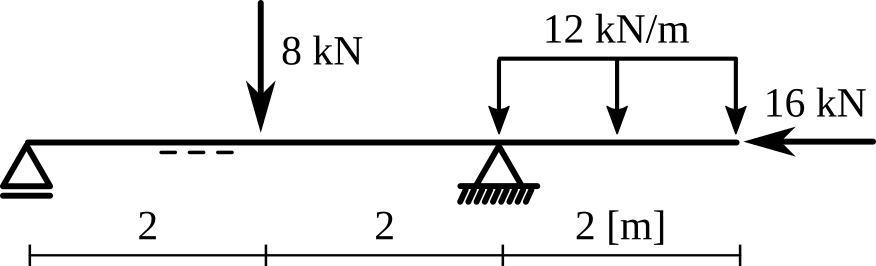
\includegraphics{Belki/Beam01.png}
    %\caption{}
\end{figure}

\begin{figure}[htbp]
    \centering
    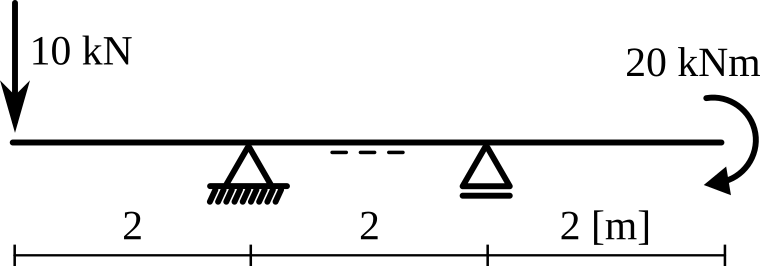
\includegraphics{Belki/Beam02.png}
    %\caption{}
\end{figure}

\begin{figure}[htbp]
    \centering
    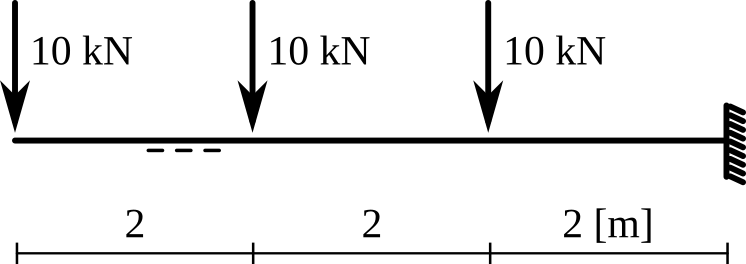
\includegraphics{Belki/Beam03.png}
    %\caption{}
\end{figure}

\begin{figure}[htbp]
    \centering
    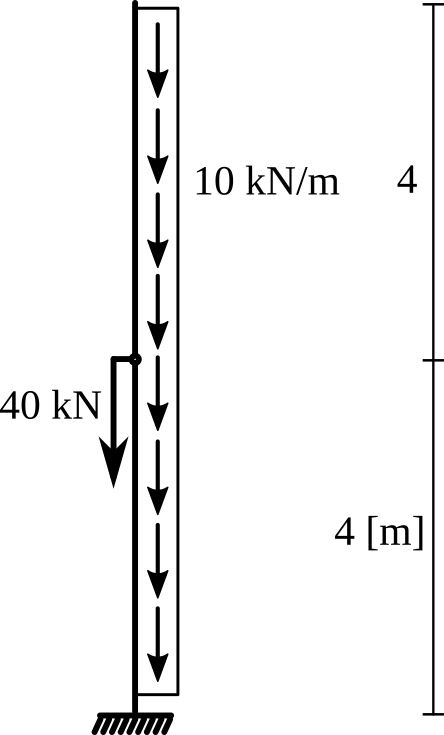
\includegraphics{Belki/Beam04.png}
    %\caption{}
\end{figure} % Zadania z sil wewnetrznych w belkach

\end{document}